\section{Result}

\subsection{Task 1 }
The first part of the goals mentioned above has been achieved using Pandas in Python by extracting periods of high-pressure blocking based on a pressure limit and a rainfall limit. The pressure limit was chosen to be \SI{1015}{\hecto\pascal}, meaning that a high-pressure blocking event must maintain at least \SI{1015}{\hecto\pascal} throughout the entire period. The rainfall limit was set to \SI{0.5}{\milli\meter}, meaning the period can have a maximum of \SI{0.5}{\milli\meter} rainfall during the entire period. The minimum period length was set to 5 days. The result during the year 2001 can be seen in \autoref{fig:2001}.

\begin{figure}[H]
    \centering    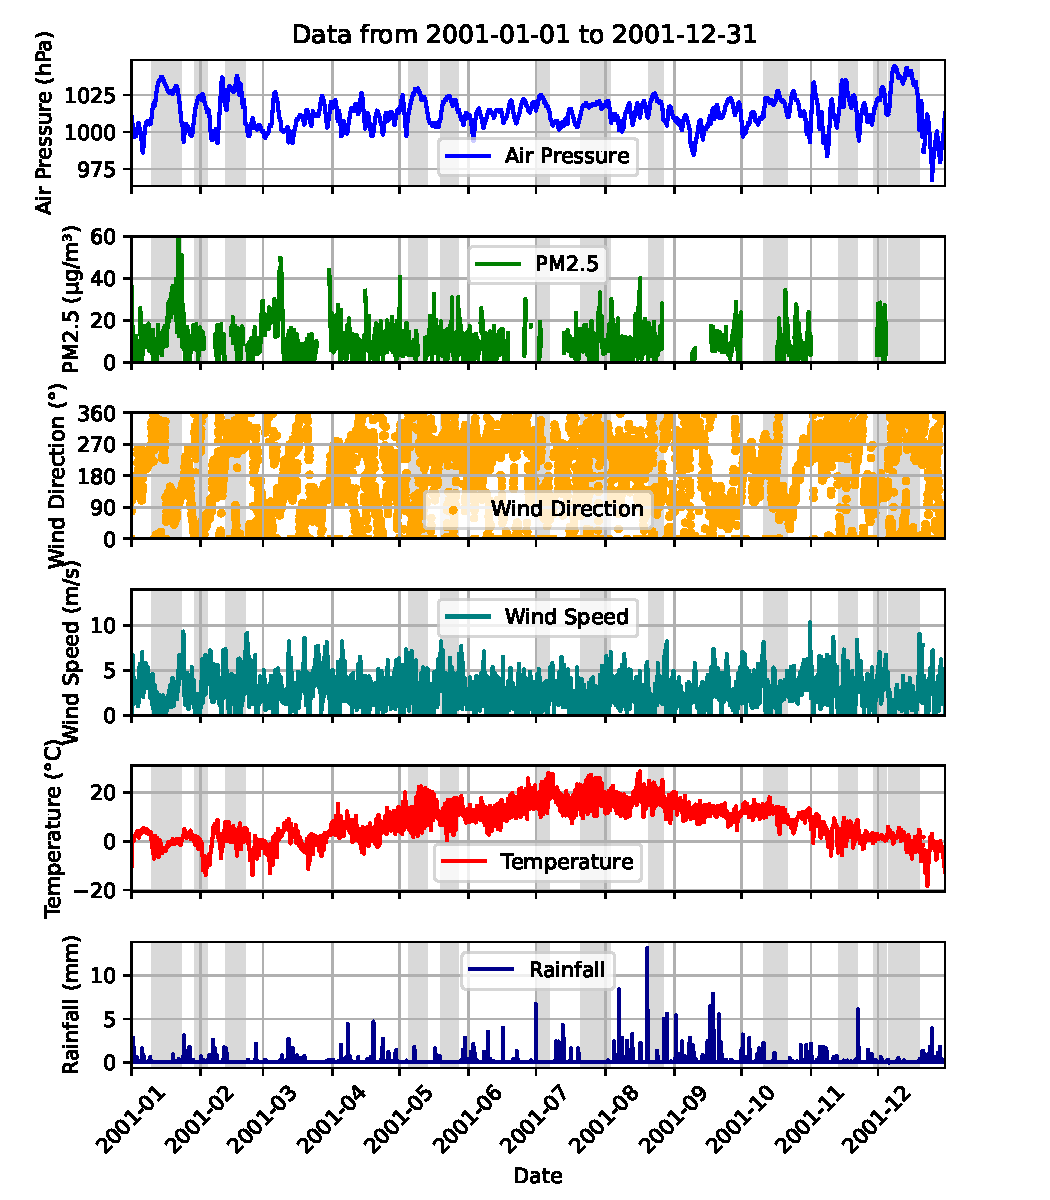
\includegraphics[width=0.7\textwidth]{Figures/plot_20010101_20011231.pdf}
    \caption{This plot displays the air pressure, PM\textsubscript{2.5} concentrations, wind direction, wind speed, temperature and rainfall during the year 2001. The periods which was filtered as periods of high pressure blocking are shown in gray. }
    \label{fig:2001}
\end{figure}

\subsection{Task 2}
The second task was to evaluate the PM\textsubscript{2.5} concentrations during periods of high pressure blocking using statistics. This was done by taking the mean of all the different blockings displaying this together with the standard deviation. This can be seen in \autoref{fig:Meanplot_Comparison}. The data is compared with the overall mean taken from the data. A slight increase in the normal concentrations of PM\textsubscript{2.5} can be seen in Malmö, while the same is hard to say about Vavihill. 





\begin{figure}[H]
    \centering
    \begin{subfigure}[b]{0.49\textwidth}
        \centering
        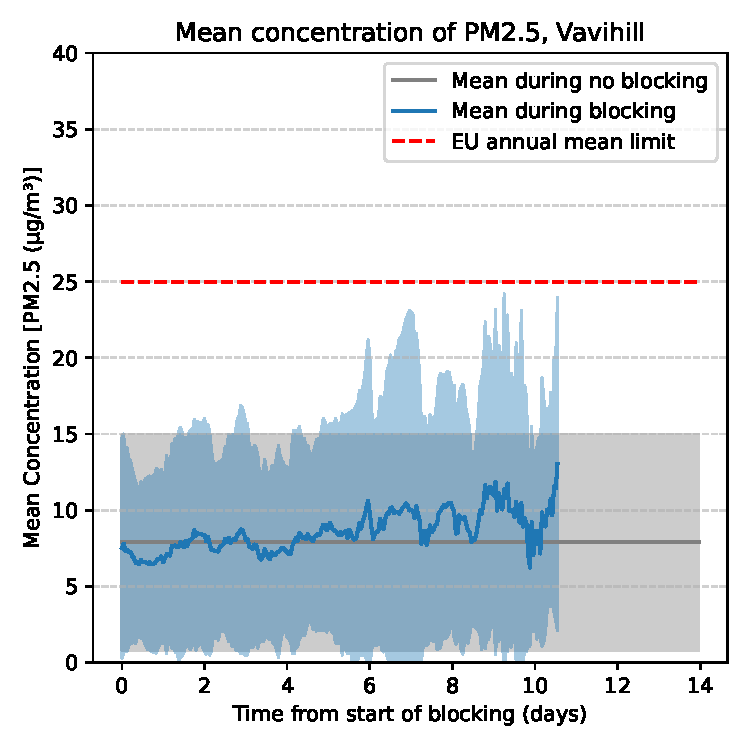
\includegraphics[width=\textwidth]{Figures/Meanplot_Vavihill.pdf}
        \caption{This figure shows the mean PM\textsubscript{2.5} concentrations over time in Vavihill. The data is analyzed to observe trends and variations in air pollution levels in a rural setting.}
        \label{fig:Meanplot_Vavihill}
    \end{subfigure}
    \hfill
    \begin{subfigure}[b]{0.49\textwidth}
        \centering
        \includegraphics[width=\textwidth]{Figures/Meanplot_Malmö.pdf}
        \caption{This figure shows the mean PM\textsubscript{2.5} concentrations over time in Malmö. The data is analyzed to observe trends and variations in air pollution levels in an urban environment.}
        \label{fig:Meanplot_Malmö}
    \end{subfigure}
    \begin{subfigure}[b]{0.49\textwidth}
        \centering
        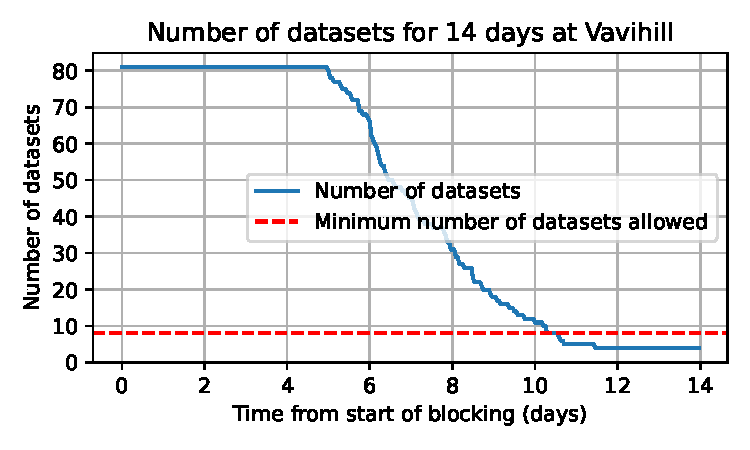
\includegraphics[width=\textwidth]{Figures/Meanplotinfo_Vavihill.pdf}
        \caption{This plot shows the number of datatsets used per day for the calculation above at Vavihill.}
        \label{fig:Meanplotinfo_Vavihill}
    \end{subfigure}
    \hfill
    \begin{subfigure}[b]{0.49\textwidth}
        \centering
        \includegraphics[width=\textwidth]{Figures/Meanplotinfo_Malmö.pdf}
        \caption{This plot shows the number of datatsets used per day for the calculation above at Malmö.}
        \label{fig:Meanplotinfo_Malmö}
    \end{subfigure}
    \caption{Comparison of mean PM\textsubscript{2.5} concentrations in Vavihill and Malmö, highlighting differences between rural and urban air quality.}
    \label{fig:Meanplot_Comparison}
\end{figure}


\autoref{fig:PM25_wind_direction} shows the increase in PM\textsubscript{2.5} concentrations in vavihill and Malmö for different wind directions. Even though the Concentration increased more in Malmö than in Vavihill, the directional dependence is less prominent.This may suggest that the accumulation of PM\textsubscript{2.5} in Malmö may be due to the local emissions in Malmö being much greater than those in Vavihill, while the increase of PM\textsubscript{2.5} in Vavihill may be more to the aerosols being transported to the area via the anticyclonic winds.  



\begin{figure}[H]
    \centering
    \begin{subfigure}[b]{0.49\textwidth}
        \centering
        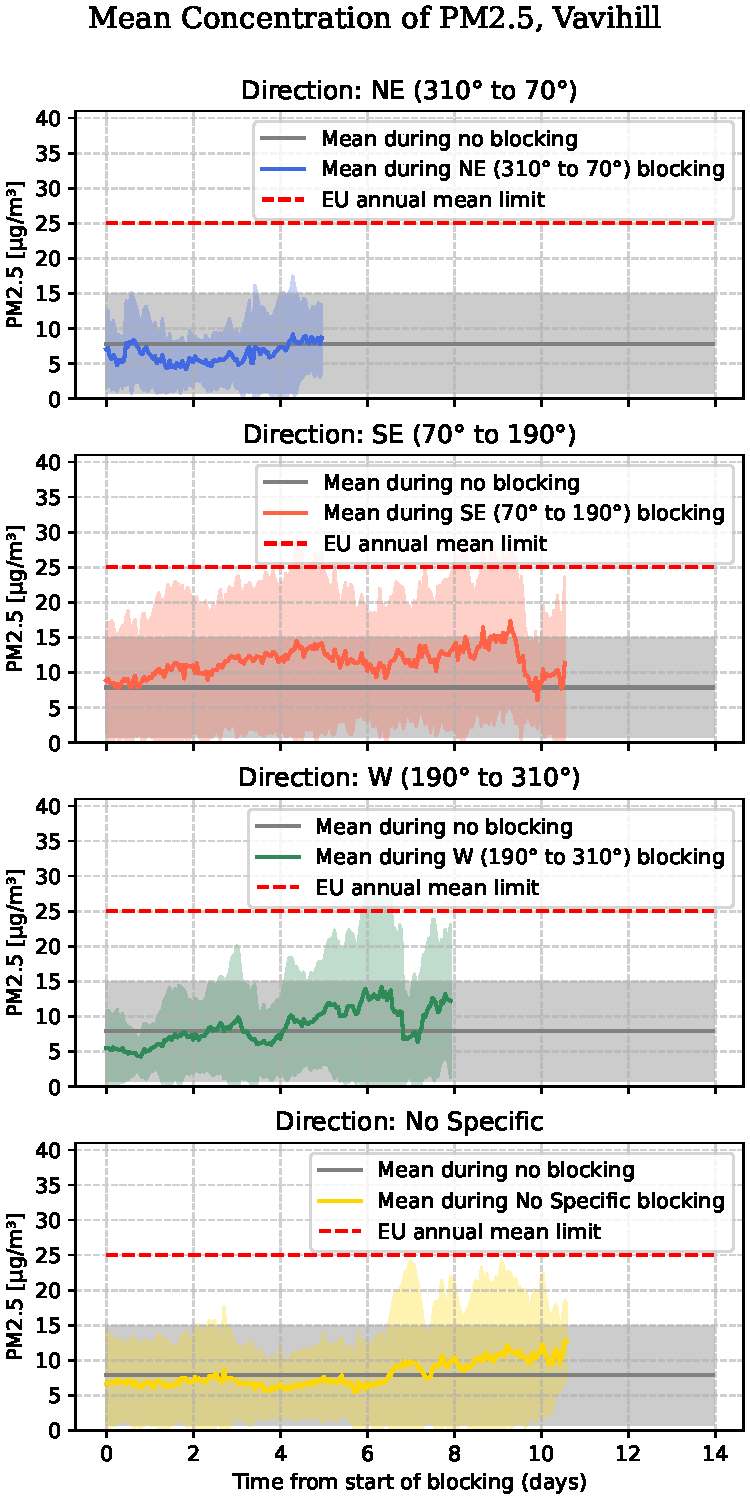
\includegraphics[width=\textwidth]{Figures/Meanplot_dir_Vavihill.pdf}
        \caption{These plots show how PM\textsubscript{2.5} concentrations change in Vavihill for different wind directions. It is important to note that 12.3\% of the winds came from the Northeast (310° to 70°), 26.6\% from the Southeast (70° to 190°), 21.4\% from the West (190° to 310°), 30.5\% from no specific direction and during 9.1\% there was no wind.}
        \label{fig:Meanplot_dir_Vavihill}
    \end{subfigure}
    \hfill
    \begin{subfigure}[b]{0.49\textwidth}
        \centering
        \includegraphics[width=\textwidth]{Figures/Meanplot_dir_Malmö.pdf}
        \caption{These plots show how PM\textsubscript{2.5} concentrations change in Malmö for different wind directions. It is important to note that 9.7\% of the winds came from the Northeast (310° to 70°), 25.3\% from the Southeast (70° to 190°), 16.2\% from the West (190° to 310°), 16.9\% from no specific direction and during 31.8\% there was no wind.}
        \label{fig:Meanplot_dir_Malmö}
    \end{subfigure}
    \caption{Comparison of PM\textsubscript{2.5} concentrations in Vavihill and Malmö for different wind directions. Note that a minimum number of datasets was still put to 8, resulting in some directions having very little data. }
    \label{fig:PM25_wind_direction}
\end{figure}

\begin{figure}[H]
    \centering
    \begin{subfigure}[b]{0.49\textwidth}
        \centering
        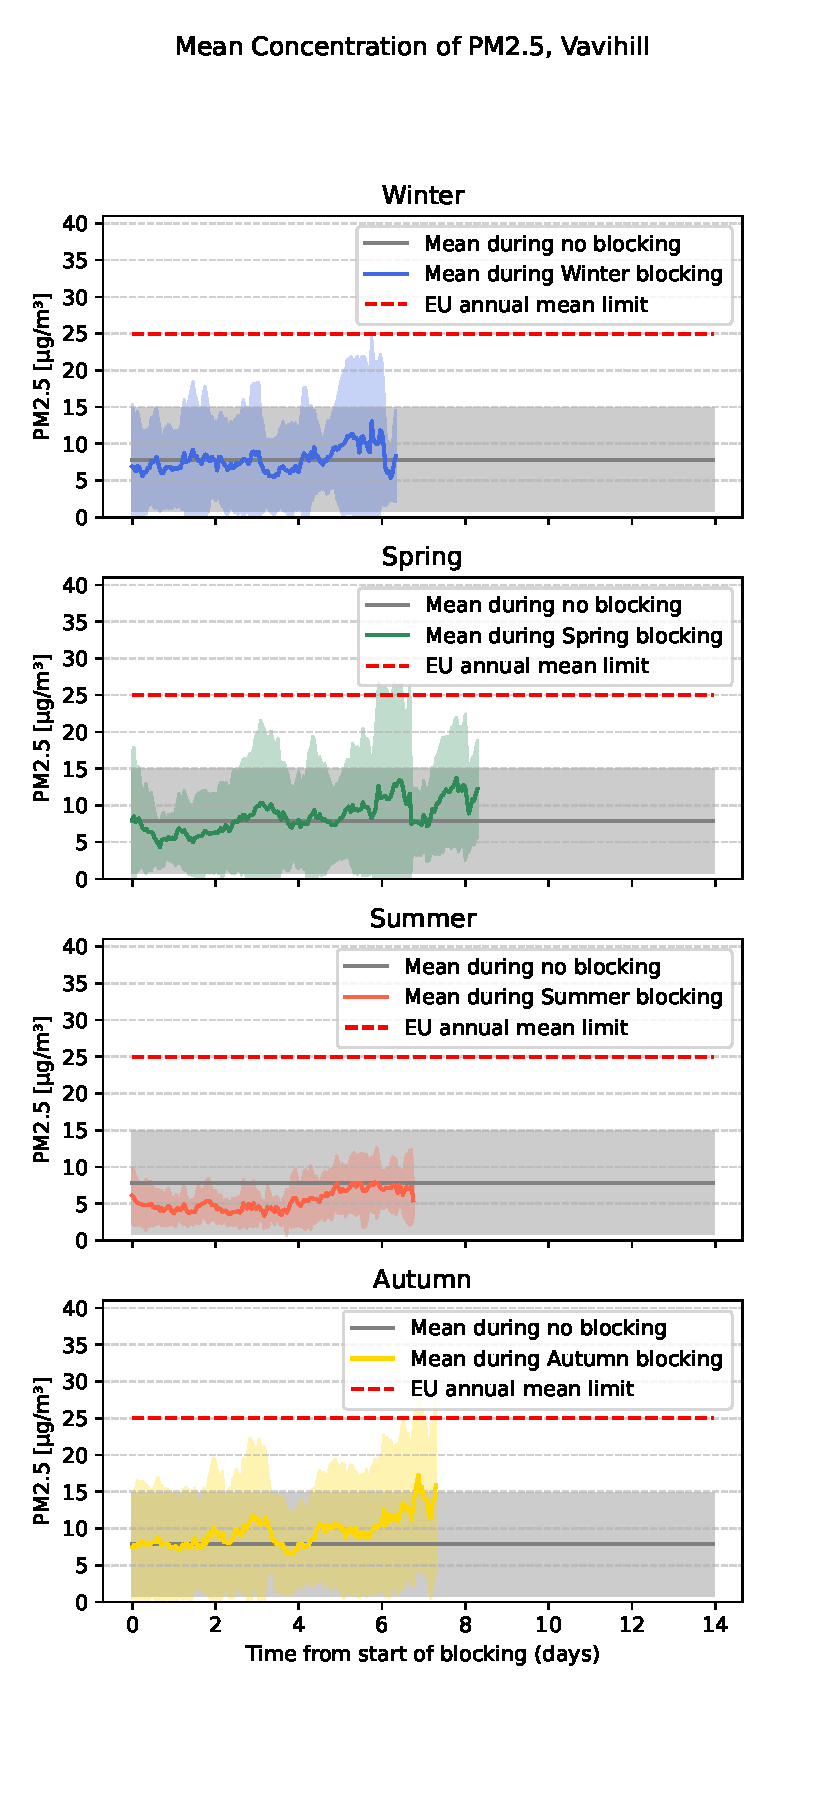
\includegraphics[width=\textwidth]{Figures/Meanplot_seasonal_Vavihill.pdf}
        \caption{These plots show how PM\textsubscript{2.5} concentrations change in Vavihill for different seasons. It is important to note that 21.3\% of the blockings occured during the winter, 37.7\% during the spring, 16.4\% during the summer and 24.6\% during the autumn.}
        \label{fig:Meanplot_seasonal_Vavihill}
    \end{subfigure}
    \hfill
    \begin{subfigure}[b]{0.49\textwidth}
        \centering
        \includegraphics[width=\textwidth]{Figures/Meanplot_seasonal_Malmö.pdf}
        \caption{These plots show how PM\textsubscript{2.5} concentrations change in Malmö for different seasons. It is important to note that 26.4\% of the blockings occurred during the winter, 33.1\% during the spring, 18.2\% during the summer and 22.3\% during the autumn.}
        \label{fig:Meanplot_seasonal_Malmö}
    \end{subfigure}
    \caption{Comparison of PM\textsubscript{2.5} concentrations in Vavihill and Malmö for different seasons. Note that a minimum number of datasets was still put to 8. }
    \label{fig:PM25_seasons}
\end{figure}


\begin{figure}[H]
    \centering
    \begin{subfigure}[b]{0.49\textwidth}
        \centering
        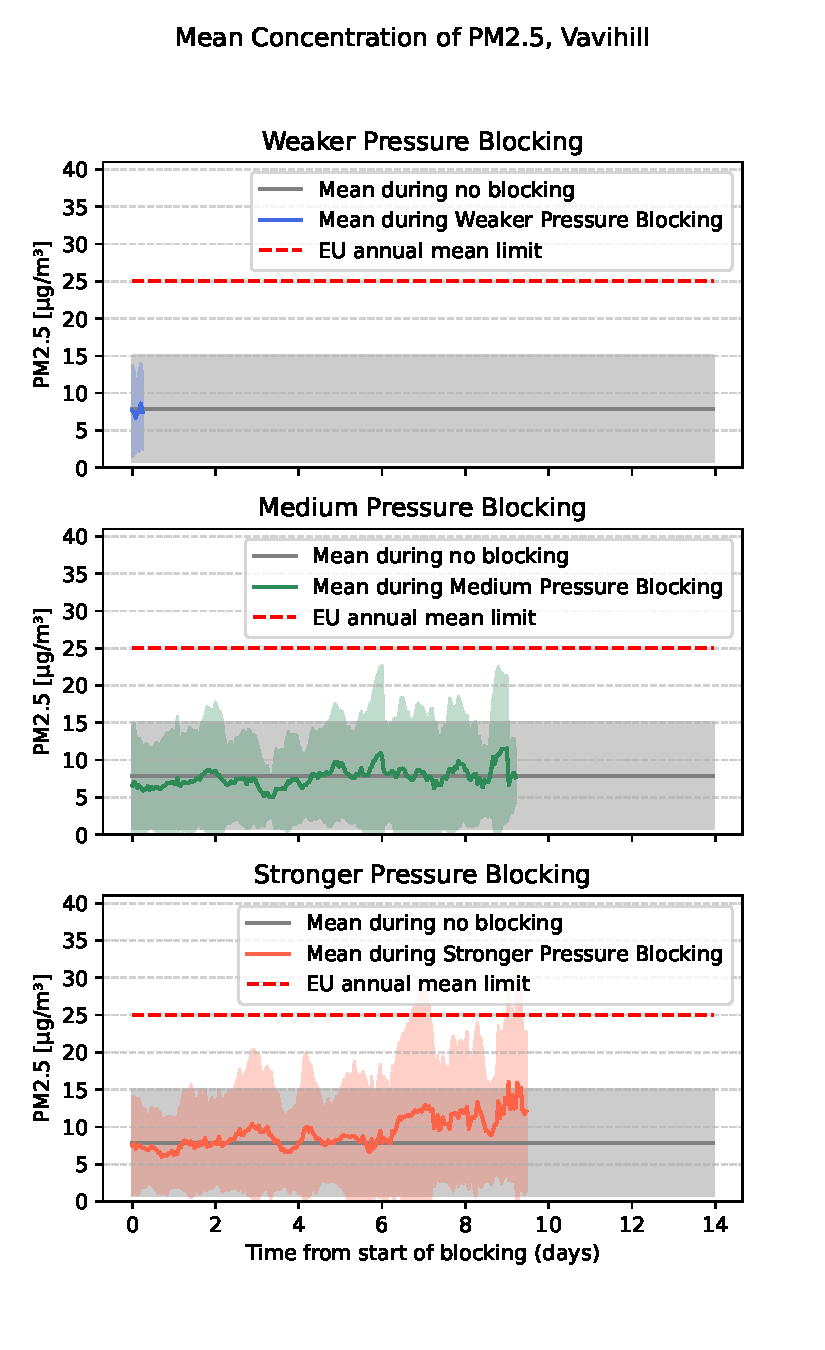
\includegraphics[width=\textwidth]{Figures/Meanplot_pressure_Vavihill.pdf}
        \caption{These plots show how PM\textsubscript{2.5} concentrations change in Vavihill for different seasons. It is important to note that 12.5\% of the blockings occurred with a mean pressure below 1020 hPa 52.8\% occurred between 1020 and 1025 hPa and 34.7\% occurred between 1025 and 1030 hPa.}
        \label{fig:Meanplot_pressure_Vavihill}
    \end{subfigure}
    \hfill
    \begin{subfigure}[b]{0.49\textwidth}
        \centering
        \includegraphics[width=\textwidth]{Figures/Meanplot_pressure_Malmö.pdf}
        \caption{These plots show how PM\textsubscript{2.5} concentrations change in Malmö for different seasons. It is important to note that 11.3\% of the blockings occurred with a mean pressure below 1020 hPa 54.2\% occurred between 1020 and 1025 hPa and 34.5\% occurred between 1025 and 1030 hPa.}
        \label{fig:Meanplot_pressure_Malmö}
    \end{subfigure}
    \caption{Comparison of PM\textsubscript{2.5} concentrations in Vavihill and Malmö for different strength of the high pressure blocking. Note that a minimum number of datasets was still put to 8. }
    \label{fig:PM25_blocking_strength}
\end{figure}

\subsection{Task 3}
The last task was to determine if the number of days under high-pressure blockings has increased, in \autoref{fig:histograms}, it can be seen that this is not the case. The seasonal dependency was also accounted for, which can be observed in the plots.


\begin{figure}[H]
    \centering
    \subfloat[Spring]{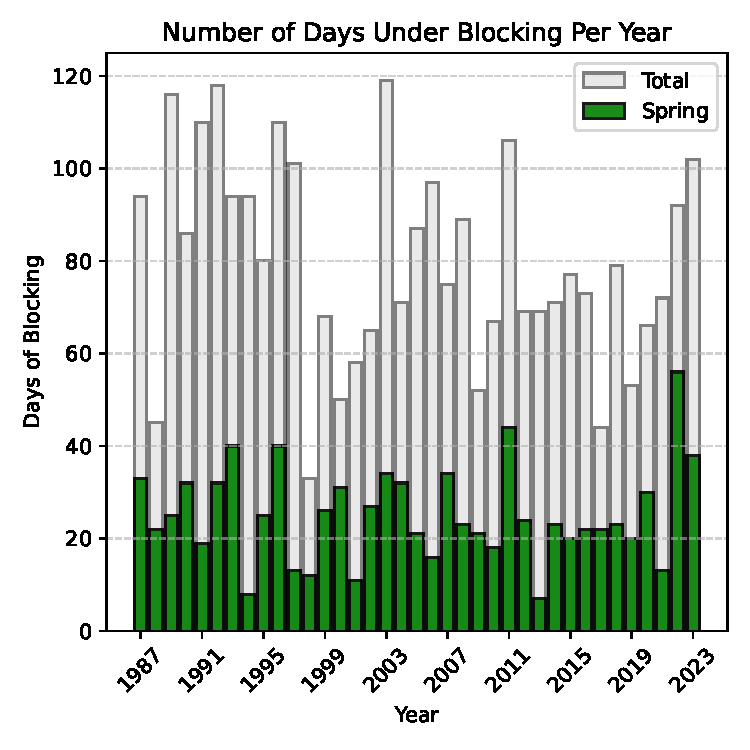
\includegraphics[width=0.49\textwidth]{Figures/Histogram_spring.pdf} \label{fig:spring}}
    \hfill
    \subfloat[Summer]{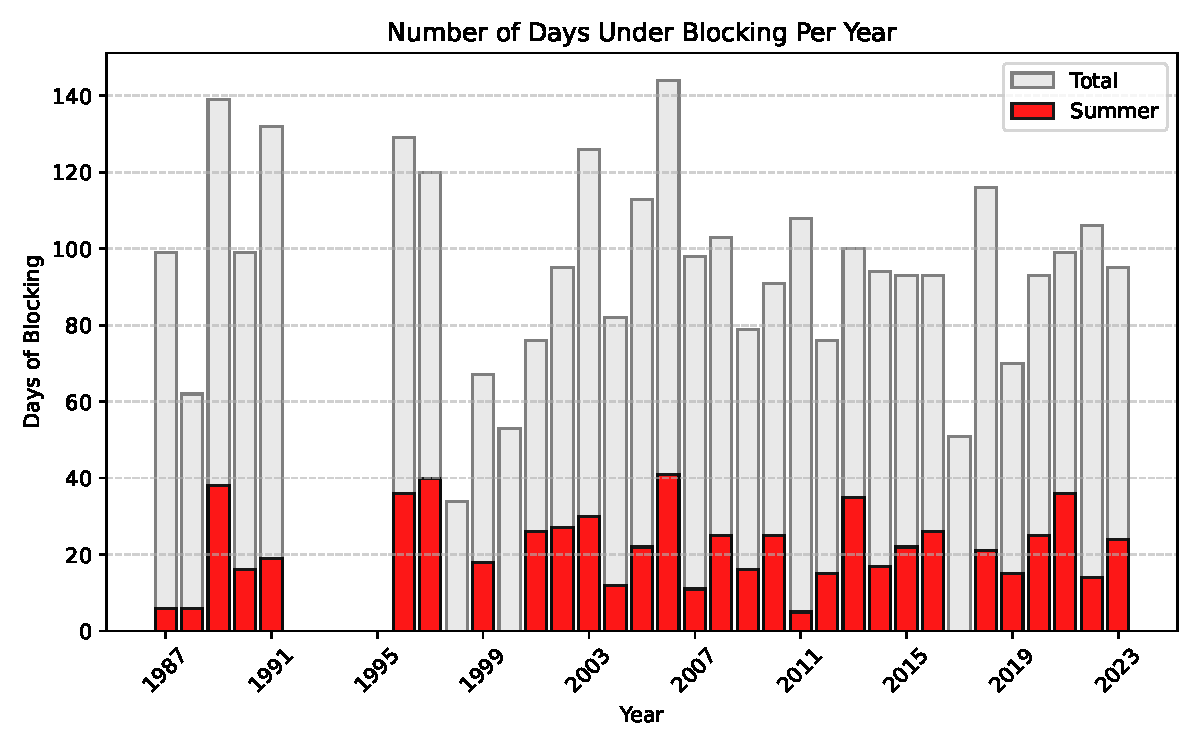
\includegraphics[width=0.49\textwidth]{Figures/Histogram_summer.pdf} \label{fig:summer}}
    
    \vspace{0.5cm}
    
    \subfloat[Autumn]{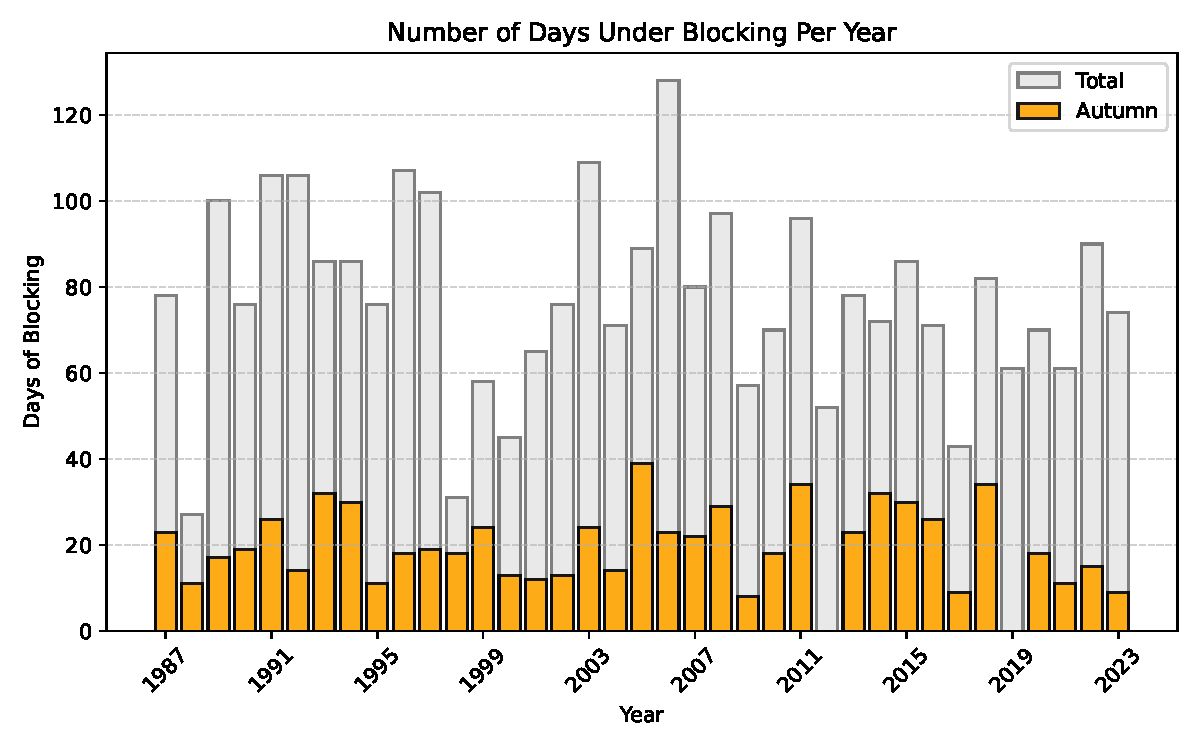
\includegraphics[width=0.49\textwidth]{Figures/Histogram_autumn.pdf} \label{fig:autumn}}
    \hfill
    \subfloat[Winter]{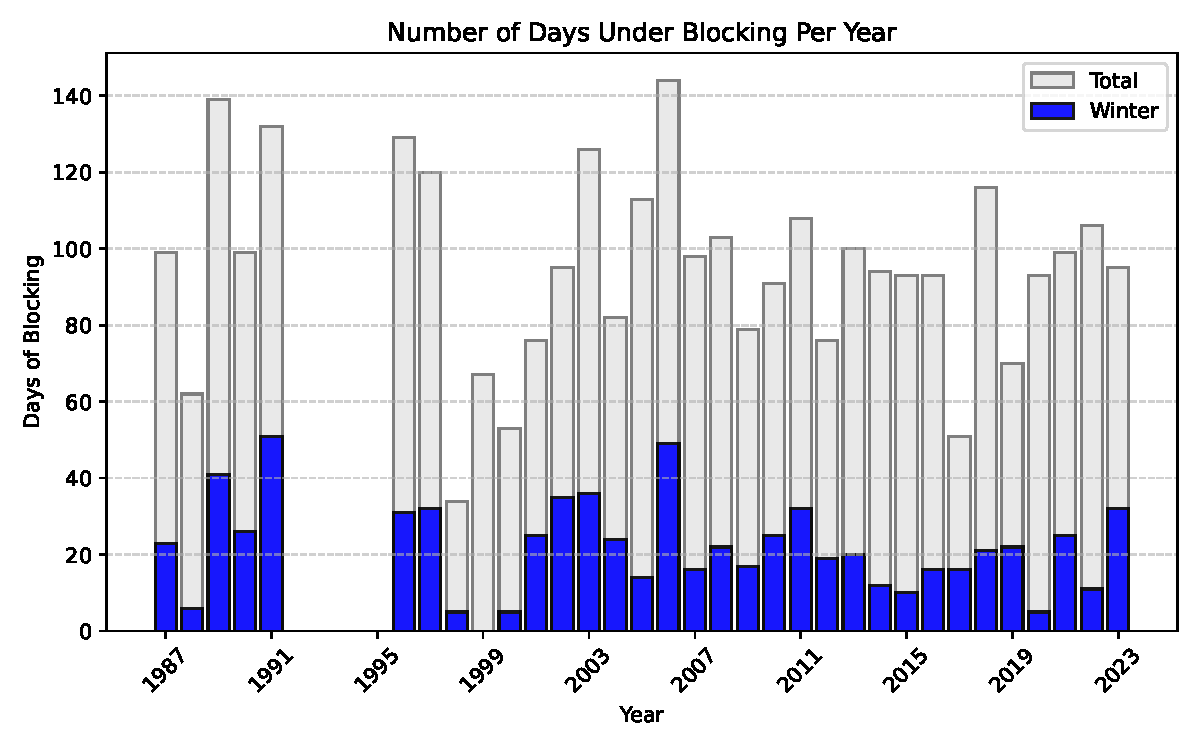
\includegraphics[width=0.49\textwidth]{Figures/Histogram_winter.pdf} \label{fig:winter}}
    
    \caption{Histograms for different seasons.}
    \label{fig:histograms}
\end{figure}
One can in \autoref{fig:blockings} see that the number of events with high pressure blocking per year has also not increased. 

\begin{figure}[H]
    \centering
    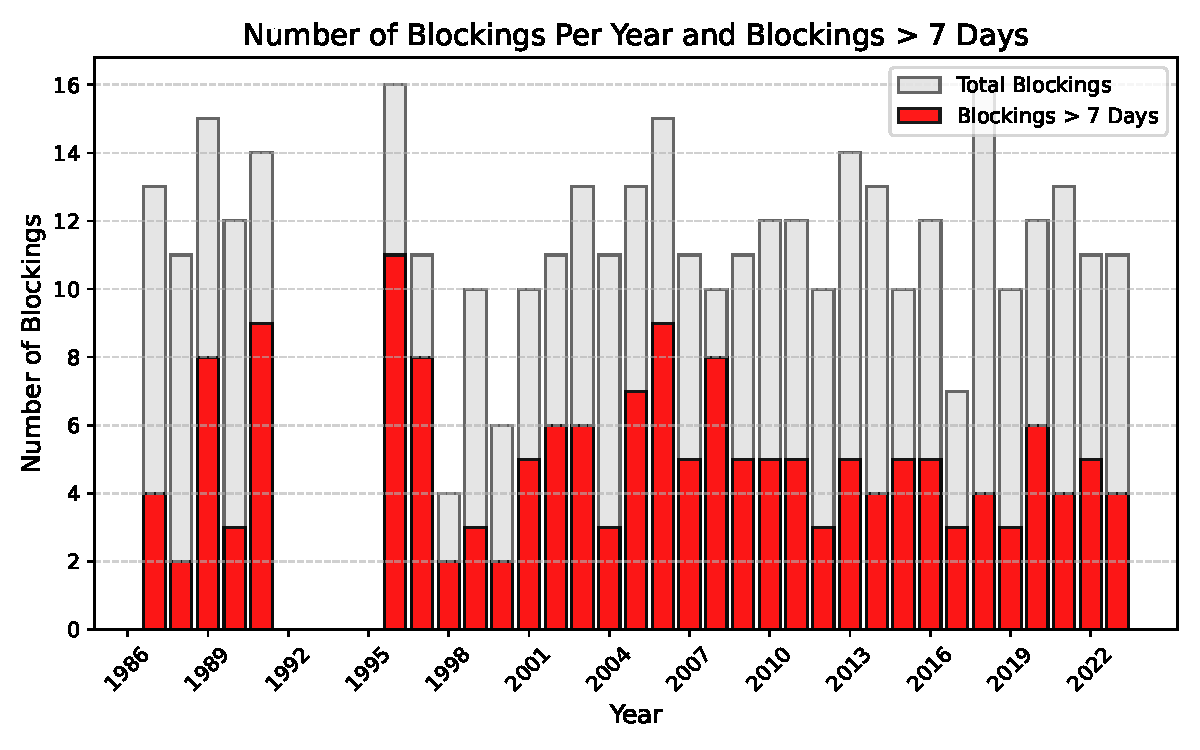
\includegraphics[width=0.7\textwidth]{Figures/BlockingsPerYear.pdf}
    \caption{This figure shows the number of high-pressure blockings per year, highlighting any trends or variations over time.}
    \label{fig:blockings}
\end{figure}




